%%%%%%%%%%%%%%%%%%%%%%% file template.tex %%%%%%%%%%%%%%%%%%%%%%%%%
%
% This is a general template file for the LaTeX package SVJour3
% for Springer journals.          Springer Heidelberg 2010/09/16
%
% Copy it to a new file with a new name and use it as the basis
% for your article. Delete % signs as needed.
%
% This template includes a few options for different layouts and
% content for various journals. Please consult a previous issue of
% your journal as needed.
%
%%%%%%%%%%%%%%%%%%%%%%%%%%%%%%%%%%%%%%%%%%%%%%%%%%%%%%%%%%%%%%%%%%%
%
% First comes an example EPS file -- just ignore it and
% proceed on the \documentclass line
% your LaTeX will extract the file if required
\begin{filecontents*}{example.eps}
%!PS-Adobe-3.0 EPSF-3.0
%%BoundingBox: 19 19 221 221
%%CreationDate: Mon Sep 29 1997
%%Creator: programmed by hand (JK)
%%EndComments
gsave
newpath
  20 20 moveto
  20 220 lineto
  220 220 lineto
  220 20 lineto
closepath
2 setlinewidth
gsave
  .4 setgray fill
grestore
stroke
grestore
\end{filecontents*}
%
\RequirePackage{fix-cm}
%
%\documentclass{svjour3}                     % onecolumn (standard format)
%\documentclass[smallcondensed]{svjour3}     % onecolumn (ditto)
\documentclass[smallextended]{svjour3}       % onecolumn (second format)
%\documentclass[twocolumn]{svjour3}          % twocolumn
%
\smartqed  % flush right qed marks, e.g. at end of proof
%
\usepackage{graphicx}
\usepackage{amsmath}              
  {
      \newtheorem{assumption}{Assumption}
  }
\usepackage{amssymb}
\usepackage{graphicx}
\usepackage{caption}
%\usepackage{subcaption}

\usepackage{color}
\definecolor{seb}{rgb}{0.9,0.9,1}
\newcommand{\Seb}[1]{
\begin{center}
\fcolorbox{seb}{seb}{\parbox[t]{0.45\textwidth}{\textbf{Seb:} #1}}
\end{center}}

%
% \usepackage{mathptmx}      % use Times fonts if available on your TeX system
%
% insert here the call for the packages your document requires
%\usepackage{latexsym}
% etc.
%
% please place your own definitions here and don't use \def but
% \newcommand{}{}
%
% Insert the name of "your journal" with
% \journalname{myjournal}
%
\begin{document}

\title{Exploitation of the Quasi-structure of the Dual Hessian for distributed MPC with Non-delayed Couplings%\thanks{Grants or other notes
%about the article that should go on the front page should be
%placed here. General acknowledgments should be placed at the end of the article.}
}
%\subtitle{Do you have a subtitle?\\ If so, write it here}

\titlerunning{Exploitation of the Quasi-structure of the Dual Hessian}        % if too long for running head

\author{Emil Klintberg         \and
        Sebastien Gros %etc.
}

%\authorrunning{Short form of author list} % if too long for running head

\institute{Emil Klintberg \at
              Chalmers Uni. of Tech., Signals and Systems \\
              H\"orsalsv\"agen 11 \\
              G\"oteborg \\
              \email{kemil@chalmers.se}           %  \\
%             \emph{Present address:} of F. Author  %  if needed
           \and
           Sebastien Gros \at
              Chalmers Uni. of Tech., Signals and Systems \\
              H\"orsalsv\"agen 11 \\
              G\"oteborg \\
               \email{grosse@chalmers.se} 
}

\date{Received: date / Accepted: date}
% The correct dates will be entered by the editor


\maketitle

\begin{abstract}
This paper studies the quasi-banded structure in the Hessian of the dual function, originating from many distributed Model Predictive Control (MPC) problems. Due to the quasi-structure, we find a banded approximation of the dual Hessian, for which structure exploiting factorization methods can be used. Moreover, we show that the approximation can be used to form a quasi-Newton method. Especially for problems with a long horizon, the quasi-Newton method can find good approximations of the Newton direction, by only considering a fraction of the elements in the dual Hessian. The quasi-structure is present when both interior-point methods and active-set methods are used to solve the subproblems.

\keywords{First keyword \and Second keyword \and More}
% \PACS{PACS code1 \and PACS code2 \and more}
% \subclass{MSC code1 \and MSC code2 \and more}
\end{abstract}

\section{Introduction}

Recently there has been a great interest invested in controlling large-scale, networked systems with Model Predictive Control (MPC). Many approaches have emerged, with the common feature that they allow for distributed computations with a limited amount of communication. This is indeed an important property since computing the MPC solutions for a large-scale problem can be intractable for a single computing unit. Moreover, when the system is geographically distributed, or when subsystems do not want to share sensitive information, it can be highly impractical to centralize the data of the problem.

Distributed MPC schemes have been proposed for various classes of control problems. In \cite{Kozma2014}, a distributed multiple shooting method is proposed to tackle large-scale nonlinear MPC problems, in \cite{Perizzato2014}, a method to tackle distributed stochastic MPC problems is proposed, whereas in \cite{Conte2013} distributed robust MPC is discussed.

Formulations of distributed MPC schemes can be divided into categories depending on the degree of communication between subsystems. Methods where no communication between the local controllers are allowed are commonly denoted as decentralized MPC. Methods belonging to this class offer great scalability, and can give a good performance when the subsystems are weakly coupled \cite{Alessio2011}, \cite{Magni2006}. However, when this is not fulfilled, the performance can be far from optimal. 

Methods where communication between subsystems are allowed, are commonly referred to as cooperative/non-cooperative MPC depending on the cost function used in the local MPC controllers \cite{Venkat2005}, \cite{Rawlings2008}, \cite{Stewart2010}. In terms of optimality, methods in this class often manage to perform better compared to cooperative MPC, but generally show a derated performance compared to the centralized formulations of the MPC problem.

%In \cite{Hult2015}, autonomous vehicles are controlled through traffic intersections.

Another promising approach to achieve distributed MPC is to formulate the MPC problem centrally and solve the underlaying optimization problem with techniques stemming from the field of distributed optimization. A commonly used technique for this purpose is to use a \emph{Lagrangian relaxation} to decompose the optimization problem into low-dimensional subproblems that can be solved independently.

%Most recent works in this context can be divided into two categories. Methods, commonly referred to as consensus methods, utilizing primal decomposition, which often show promising results for very large problems with simple constraints and non-fixed network topologies \cite{}, \cite{}. The other commonly used technique for this purpose is dual decomposition where a \emph{Lagrangian relaxation} is used to decompose the optimization problem into low-dimensional subproblems that can be solved independently.

Lagrangian relaxation is used in many different contexts to tackle convex large-scale problems, e.g. the authors in \cite{Cottle1986} propose a coordinate ascent approach to solve matrix problems. In \cite{Lasdon1970}, \cite{Giselsson2010} a gradient method, whereas in \cite{Richter2011}, \cite{Necoara2011}, \cite{Giselsson2013}, \cite{Giselsson2014a}, \cite{Giselsson2014b} a fast gradient method is used in order to attain dual optimality. Moreover, in \cite{Necoara2014a}, \cite{Necoara2014b}, convergence rates for first-order methods are studied. All these methods make use of only first-order derivatives when finding a search direction.

Methods using second-order derivatives offer advantages in terms of convergence speed. In the context of active-set methods, this is exploited by the authors in \cite{Ferreau2012b}, \cite{Kozma2013a}, \cite{Kozma2014a}, \cite{Frasch2014}, \cite{Gros2014a}. However, the dual function is non-smooth and the dual Hessian can be singular if a poor initial guess is used for the dual variables, and hence possibly leading to an inconsistent Newton system. In \cite{Kozma2014a}, this issue was avoided by relaxing the local inequality constraints with an $L_2$-penalty.

In \cite{Necoara2009a}, it was proved that adding self-concordant barrier terms to the Lagrange function of a generic convex problem render a self-concordant dual function. Hence, in the context of interior-point methods, it is possible to use the Newton method to efficiently solve the dual problem. This result was used in \cite{Quoc2013}, where a method based on inexact solutions of the local subproblems was proposed. Moreover, in \cite{Klintberg2014}, a primal-dual interior-point method was proposed, which supports linear predictors and inexact solutions and showed a fast and consistent practical convergence.

Indeed, methods using second-order information offer a fast convergence in terms of iterations. However, this comes to the cost of factorizing the Hessian of the dual function at each iteration. Typically the cost of performing this factorization is cubic with respect to the dimensions of the dual space, and can hence be a bottleneck when solving large-scale problems. For specific applications, the dual Hessian can be structured and the cost of factorizing it can therefore be lowered. In the context of subproblems connected in a chain, this is exploited in \cite{Frasch2014}. However, most problems render a dense dual Hessian.

In this paper, we show that the dual Hessian of optimization problems originating from many MPC schemes have an inherent quasi-structure. The quasi-structure can be used to find a banded approximation of the dual Hessian, which offer a substantially lower cost of factorization. Hence, a quasi-Newton method can be formed which can solve many MPC problems to a lower overall complexity. The method performs especially well on problems with a very long horizon, which otherwise are challenging due to the size of the dual Hessian.

The quasi-structure arises when distributed systems, with non-delayed interactions between subsystems, are controlled with MPC. As an illustrative example, the structure will be analyzed in the context of the interior-point method described in \cite{Necoara2009a}. It should however be understood that the dual Hessian of the methods described in \cite{Quoc2013} and \cite{Klintberg2014} take the same form. For completeness, we also give a short description of the quasi-structure for active-set methods.

The paper is organized as follows. In Section \ref{S:Preliminaries}, the considered class of problems will be introduced and the dual decomposition approach with second-order derivatives will be recalled, where emphasis will be placed on the computation of the Hessian of the dual function. In Section \ref{S:TheoreticalDecay}, the quasi-banded structure of the dual Hessian is investigated. It is shown that the quasi-structure can be used to form a banded approximation of the dual Hessian, for which structure exploiting factorization methods can be used. Moreover, a quasi-Newton method based on the approximation of the dual Hessian is proposed. In Section \ref{S:ActiveSet}, the quasi-structure is briefly described in the context of active-set methods. In Section \ref{S:NumericalExperiments}, numerical experiments are performed on two examples. Features of the quasi-structure are shown and convergence properties of the quasi-Newton method are presented. The paper is concluded in Section \ref{S:Conclusions}.

\subsection{Contributions} This paper contain three contributions:
\begin{enumerate}
\item We establish that the Hessian of the dual function that is resulting from many MPC problems has a quasi-banded structure.
\item As a result of the quasi-structure, we show that the dual Hessian can be approximated by a banded matrix for which structure exploiting factorization methods can be used.
\item We show that the quasi-structure can be used to form a quasi-Newton method, where a good approximation of the Newton direction can be found by only considering a small fraction of the elements in the dual Hessian.
\end{enumerate}

\subsection{Notations} 
The notation $\mathbb{R}_{++}^{n \times m}$ (and $\mathbb{R}_{+}^{n \times m}$) defines the set of positive definite (and positive semidefinite) matrices with dimension $n \times m$. The set of symmetric matrices of dimension $n \times n$ is denoted by $\mathbb{S}^n$.

For a function $f$ with two arguments, $t \in \mathbb{R}$ and $x \in \mathbb{R}^n$, we denote the partial derivative of $f(x,t)$ w.r.t. $t$ as $f'(x,t)$ and w.r.t. $x$ as $\nabla f(x,t)$.

%In \cite{Wei2013}, a distributed Newton method is proposed to maximize network utilization.

\section{Prelimenaries} \label{S:Preliminaries}

In this section, we present the considered class of problems and recall the second-order dual decomposition approach.

\subsection{Problem formulation}
In this section, we present the class of distributed Quadratic Programs (QPs) considered in this paper. Moreover, we show how problems belonging to this class arise when MPC is used to control multiple linear systems interacting via non-delayed couplings.

Let us consider $M$ discrete time, possibly time varying, linear systems:
\begin{equation} \label{e:SystemDynamics}
x_{k,i+1} = A_{k,i} x_{k,i} + B_{k,i} u_{k,i}, \quad k = 1, \dots, M
\end{equation}
where $x_{k,i} \in \mathbb{R}^{p_{k}}$ and $u_{k,i} \in \mathbb{R}^{m_{k}}$ represents the state and input of system $k$ at time instance $i$. Moreover, each system is subject to local state and input constraints:
\begin{subequations} \label{e:StateInputConstraints}
\begin{align}
x_{k,i} \in \mathcal{X}_{k,i} \subseteq \mathbb{R}^{p_{k}}, \quad k = 1, \dots, M \\
u_{k,i} \in \mathcal{U}_{k,i} \subseteq \mathbb{R}^{m_{k}}, \quad k = 1, \dots, M
\end{align}
\end{subequations}
We assume, in this paper, that the systems interact with static, non-delayed couplings, i.e.:
\begin{equation} \label{e:MPCcouplings}
h_i(x_{1,i}, u_{1,i}, \dots, x_{M,i}, u_{M,i}) = 0, \quad i = 0,\dots,N
\end{equation}
Observe that with non-delayed couplings, we refer to interactions where states and inputs for a subsystem at time $i$ can only have a direct impact on states and inputs of another subsystem at time $i$. The interactions between the systems can accordingly not include dynamic relationships or time-delays. However, it should be understood that this can always be fulfilled by introducing extra states to handle the delays locally, even when delayed couplings are present in the original formulation.

Furthermore, let us assume that the the constraints (\ref{e:StateInputConstraints}) are convex polytopes, and that the non-delayed couplings (\ref{e:MPCcouplings}) are affine. In the following, we use the notation: $z_{k,i} = [x_{k,i}^T \quad u_{k,i}^T]^T \in \mathbb{R}^{n_{k}}$, representing the optimization variables. Using a quadratic objective function, the \emph{finite-time optimal control problem} over the horizon $N$, can then be stated as:
\begin{subequations}
\label{e:problem}
\begin{align}
\min_z & \quad \sum_{k=1}^{M} \sum_{i=0}^N \frac{1}{2}z_{k,i}^TH_{k,i}z_{k,i} + c_{k,i}^Tz_{k,i} \label{e:1} \\
\text{s.t.} & \quad \sum_{k=1}^{M} F_{k,i}z_{k,i} = e_i \label{e:CoupConstControl} \\
& C_{k,i}z_{k,i} + D_{k,i+1}z_{k,i+1} = d_{k,i} \label{e:dynamics} \\
& G_{k,i}z_{k,i} \leq f_{k,i}
\end{align}
\end{subequations}
where $H_{k,i} \in \mathbb{S}_{++}^{n_{k}}$ and $c_{k,i} \in \mathbb{R}^{n_k}$, the dynamics (\ref{e:SystemDynamics}) are described by $C_{k,i} \in \mathbb{R}^{l_{k} \times n_{k}}$, $D_{k,i+1} \in \mathbb{R}^{l_{k} \times n_{k}}$ and $d_{k,i} \in \mathbb{R}^{l_{k}}$, $F_{k,i} \in \mathbb{R}^{r_{i} \times n_{k}}$ and $e_i \in \mathbb{R}^{r_i}$ yield the non-delayed coupling constraints (\ref{e:MPCcouplings}), $G_{k,i} \in \mathbb{R}^{t_{k} \times n_{k}}$ and $f_{k,i} \in \mathbb{R}^{t_{k}}$ form the local state and input constraints (\ref{e:StateInputConstraints}).

Additionaly, to avoid unnecessarily heavy notation, we introduce the following augmented notations: $z_k = [z_{k,0}^T \dots, z_{k,N}^T]^T \in \mathbb{R}^{(N+1)n_k}$, which represents the collection of states and inputs of system $k$ over the horizon $N$. The MPC problem (\ref{e:problem}) can then be expressed as:
\begin{subequations}
\label{e:problem1}
\begin{align}
\min_z & \quad \sum_{k=1}^{M} \frac{1}{2}z_k^TH_k z_k + c_k^Tz_k \label{e:1} \\
\text{s.t.} & \quad \sum_{k=1}^{M} F_k z_k = e \label{e:CoupConst} \\
& C_k z_k = d_k \label{e:3} \\
& G_k z_k \leq f_k \label{e:ineqConst}
\end{align}
\end{subequations}
where $H_{k} \in \mathbb{S}_{++}^{(N+1)n_{k} \times (N+1)n_{k}}$, $C_{k} \in \mathbb{R}^{N l_{k} \times (N+1)n_{k}}$ and $d_{k} \in \mathbb{R}^{N l_{k}}$, $F_{k} \in \mathbb{R}^{(N+1) r \times (N+1) n_{k}}$ and $e \in \mathbb{R}^{(N+1)r}$, $G_{k} \in \mathbb{R}^{(N+1) t_{k} \times (N+1) n_{k}}$ and $f_{k} \in \mathbb{R}^{(N+1) t_{k}}$.

The matrices in (\ref{e:problem1}) possess banded structures given by:
\begin{subequations}
\begin{align}
& H_k = \left[ \begin{array}{ccc}
H_{k,0} & & \\
 & \ddots & \\
 & & H_{k,N}
\end{array} \right], \\
& F_k = \left[ \begin{array}{ccc}
F_{k,0} & & \\
 & \ddots & \\
 & & F_{k,N}
\end{array} \right], \\
& C_k = \left[ \begin{array}{ccccc} 
C_{k,0} & D_{k,1} &  &   &  \\
 & C_{k,1} & D_{k,2} &  &  \\
 &  & \ddots & \ddots &  \\
 &  &  & C_{k,N-1} & D_{k,N}
\end{array} \right], \label{e:C} \\
& A_k = \left[ \begin{array}{ccc}
A_{k,0} & & \\
 & \ddots & \\
 & & A_{k,N}
\end{array} \right].
\end{align}
\end{subequations}
These banded structures will be key elements for the quasi-banded structure of the dual Hessian.

\subsection{Dual decomposition with second-order information} \label{s:DualDecomposition}
In this section, we introduce the second-order dual decomposition approach. The aim is to present a constraint relaxation, first described in \cite{Necoara2009a}, in order to make the dual function self-concordant. Self-concordance is an important property for constructing polynomial time interior-point methods \cite{Nesterov1994}, and is hence a desirable feature since Newton steps in the dual space are considered. We detail next the construction of the dual Hessian, which is needed in order to compute a Newton step.

We introduce the dual variables $\lambda \in \mathbb{R}^{(N+1) r}$ corresponding to the coupling constraints (\ref{e:CoupConst}) and define the Lagrange function as:
\begin{equation}
\mathcal{L}(z,\lambda) =  \sum_{k=1}^{M} ( \frac{1}{2}z_k^TH_kz_k + c_k^Tz_k ) + \lambda^T ( \sum_{k=1}^{M} F_k z_k - e )
\end{equation}
We observe that $\mathcal{L}(z,\lambda)$ is separable in $z$, i.e.:
\begin{equation}
\mathcal{L}(z,\lambda) = \sum_{k=1}^{M} \mathcal{L}_k (z_k,\lambda),
\end{equation}
with:
\begin{equation}
\mathcal{L}_k(z_k,\lambda) = \frac{1}{2}z_k^TH_k z_k + c_k^T z_k + \lambda^T(F_k z_k - \frac{1}{M} e),
\end{equation}
such that the dual function $d(\lambda) = -\min_{z \in \mathcal{Z}} \mathcal{L}(z,\lambda)$ can be evaluated in parallel as:
\begin{equation}
\label{e:dualfunction}
d(\lambda) = -\sum_{k=1}^M \min_{z_k \in \mathcal{Z}_k} \mathcal{L}_k(z_k,\lambda)
\end{equation}

Since (\ref{e:problem1}) is strictly convex, $d(\lambda)$ is convex and continuously differentiable, but not twice differentiable \cite{Kozma2014a}. However, the Hessian of $d(\lambda)$ is a constant matrix over any fixed active-set of (\ref{e:problem}) \cite{Kozma2014a}.

As a result, $d(\lambda)$ is not self-concordant and the solution to the dual problem is not easily tracked with the Newton method. However, if the inequality constraints (\ref{e:ineqConst}) are relaxed with a self-concordant log-barrier, according to:
\begin{subequations}
\label{e:relaxedproblem}
\begin{align}
\min_z & \quad \sum_{k=1}^{M} \frac{1}{2}z_k^TH_k z_k + c_k^T z_k - \tau \sum_{i=1}^{(N+1)t_k} \log([s_k]_i) \label{e:1} \\
\text{s.t.} & \quad \sum_{k=1}^{M} F_k z_k = e \\
& \quad C_k z_k = d_k \\
& \quad G_k z_k + s_k = f_k
\end{align}
\end{subequations}
where $\tau > 0$ will be referred to as the \emph{barrier parameter}, the resulting \emph{relaxed dual function} $d(\lambda, \tau)$ is self-concordant \cite{Necoara2009a}. As a result, a sequence of dual problems $\left\{\min_\lambda d(\lambda, \tau) \right\}_{\tau \rightarrow 0}$ can be solved, where each problem is self-concordant and therefore easily handled with the Newton method. The \emph{relaxed dual function} can be made to be an arbitrary good approximation of (\ref{e:dualfunction}) by making $\tau$ arbitrary small.

In contrast to smoothing techniques based on the \emph{augmented Lagrangian} \cite{Kozma2013}, the separability of the dual function is preserved, and the relaxed dual function can be computed in parallel using:
\begin{equation}
\label{e:relaxeddualfunction}
d(\lambda, \tau) = -\sum_{k=1}^M \min_{z_k \in \mathcal{Z}_k} \left( \mathcal{L}_k(z_k, \lambda) - \tau \sum_{i=1}^{m_k} \log([s_k]_i) \right)
\end{equation}
Observe that evaluating (\ref{e:relaxeddualfunction}) involves solving $M$ independent subproblems of the form:
\begin{equation}
\label{e:localproblem}
\begin{aligned}
\min_{z_k} & \quad \frac{1}{2}z_k^T H_k z_k + c_k^T z_k + \lambda^TF_k z_k - \tau \sum_{i=1}^{m_k} \log([s_k]_i) \\
\text{s.t.} & \quad C_k z_k = d_k \\ 
& \quad G_k z_k + s_k = f_k \\
& \quad s_k \geq 0
\end{aligned}
\end{equation}

Strict convexity of (\ref{e:relaxedproblem}) implies that the gradient of $d(\lambda, \tau)$ with respect to $\lambda$ is given by the residual of the coupling constraints \cite{Bertsekas1989}, i.e.:
\begin{equation}
\label{e:dualgradient}
\nabla d(\lambda, \tau) = -\sum_{k=1}^M F_k z_k^*(\lambda, \tau) + e
\end{equation}
where $z_k^*(\lambda, \tau)$ is the solution to (\ref{e:localproblem}).
The dual Hessian is then given by:
\begin{equation}
\label{e:dualhessian}
\nabla^2 d(\lambda, \tau) = -\sum_{k=1}^M F_k \frac{\partial z_k^*(\lambda, \tau)}{\partial \lambda}
\end{equation}

Recall that in order to find the solution $\lambda^*(\tau)$ to the dual problem $\min_\lambda d(\lambda, \tau)$, $\lambda$ is updated by taking Newton steps $\Delta \lambda$. A Newton step in the dual space can be obtained as a solution to the Newton system:
\begin{equation}
\label{e:NewtonSystem}
\nabla^2 d(\lambda, \tau) \Delta \lambda + \nabla d(\lambda, \tau) = 0
\end{equation}

Finding the Newton step requires knowledge of the gradient and the Hessian of the dual function $d(\lambda, \tau)$. Note that the dual gradient (\ref{e:dualgradient}) can be easily computed from the solutions $z_k^*(\lambda, \tau)$ to (\ref{e:localproblem}), while the Hessian (\ref{e:dualhessian}) requires the sensitivities $\frac{\partial z_k^*(\lambda, \tau)}{\partial \Lambda}$. In the following, we will describe how $\frac{\partial z_k^*(\lambda, \tau)}{\partial \Lambda}$ can be computed, for a detailed description we refer to \cite{Klintberg2014}.

By introducing $y_k = \tau s_k^{-1} \in \mathbb{R}^{t_k (N + 1)}$, the primal-dual interior point KKT conditions to (\ref{e:localproblem}) can be stated as:
\begin{subequations} \label{e:KKTconditions}
\begin{align}
& 0 = H_k z_k^* + c_k + F_k^T \lambda + C_k^T \mu_k^* + G_k^T y_k^* \\
& 0 = C_k z_k^* - d_k \\
& 0 = G_k z_k^* + s_k^* - f_k \\
& 0 = Y_k^* s_k^* - \tau \mathbf{1} \\
& s_k^* > 0, \quad y_k^* > 0
\end{align}
\end{subequations}
By differentiating (\ref{e:KKTconditions}), the following linear system is obtained \cite{Klintberg2014}:
\begin{equation}
\label{e:SensitivityLambda}
\left[ \begin{array}{cccc}
H_k & C_k^T & G_k^T & 0 \\
C_k & 0 & 0 & 0 \\
G_k & 0 & 0 & I \\
0 & 0 & S_k & Y_k
\end{array} \right]
\left[ \begin{array}{c}
\frac{\partial z_k^*}{\partial \lambda} \\
\frac{\partial \mu_k^*}{\partial \lambda} \\
\frac{\partial y_k^*}{\partial \lambda} \\
\frac{\partial s_k^*}{\partial \lambda}
\end{array} \right] = -
\left[ \begin{array}{c}
F_k^T \\
0 \\
0 \\
0
\end{array} \right]
\end{equation}
From the primal sensitivity, $\frac{\partial z_k^*(\lambda, \tau)}{\partial \lambda}$, the dual Hessian can then be formed according to (\ref{e:dualhessian}).

\section{Quasi-structure of the dual Hessian} \label{S:TheoreticalDecay}

In this section, we show that the dual Hessian decays exponentially towards its off-diagonal corners, and hence possess a quasi-banded structure. We derive theoretical bounds on the magnitude of its elements. Moreover, we propose a quasi-Newton method based on a banded approximation of the dual Hessian.

\subsection{Quasi-banded} \label{s:QuasiBanded}
In Section \ref{s:DualDecomposition}, we presented a way of computing the dual Hessian. In this section, we will detail its properties by forming an explicit expression and characterizing its quasi-banded structure. The quasi-banded structure allows to approximating the dual Hessian by a banded matrix, for which structure exploiting factorization methods can be used.

The analysis of the structure will be based on the explicit expression of the dual Hessian, stated in the following proposition:
\begin{proposition}
The Hessian of the dual function $d(\lambda, \tau)$ is given by:
\begin{equation}
\label{e:dualhessian2}
\nabla^2 d(\lambda, \tau) = \sum_{k=1}^M F_k (\Phi_k^{-1} - \Phi_k^{-1} C_k^T \Lambda_k^{-1} C_k \Phi_k^{-1}) F_k^T
\end{equation}
where
\begin{align}
& \Phi_k = H_k + G_k^T S_k^{-1} Y_k G_k \label{e:Phi} \\
& \Lambda_k = C_k \Phi_k^{-1} C_k^{T} \label{e:Lambda}
\end{align}
\end{proposition}
\begin{proof}
By using block elimination of (\ref{e:SensitivityLambda}), it can be obtained that:
\begin{subequations}
\begin{align}
& \Lambda_k (s_k, y_k) \frac{\partial \mu_k^*}{\partial \lambda} = -C_k \Phi_k^{-1} F_k^T \label{e:firstNormalEquation} \\
& \Phi_k (s_k, y_k) \frac{\partial z_k^*}{\partial \lambda} = -F_k^T - C_k^T \frac{\partial \mu_k^*}{\partial \lambda} \label{e:secondNormalEquation}
\end{align}
\end{subequations}
where
\begin{subequations}
\begin{align}
& \Phi_k (s_k, y_k) = H_k + G_k^T S_k^{-1} Y_k G_k \in \mathbb{S}_{++}^{(N+1)n_k \times (N+1)n_k} \\
& \Lambda_k (s_k, y_k) = C_k \Phi_k^{-1}(s_k, y_k) C_k^{T} \in \mathbb{S}_{++}^{N l_k \times N l_k} \label{e:Lambda}
\end{align}
\end{subequations}
By using (\ref{e:firstNormalEquation}) to eliminate $\frac{\partial \mu_k^*}{\partial \lambda}$ in (\ref{e:secondNormalEquation}), the following is obtained:
\begin{equation}
\label{e:localcontributions}
F_k \frac{\partial z_k^*}{\partial \lambda} = -F_k (\Phi_k^{-1} - \Phi_k^{-1} C_k^T \Lambda_k^{-1} C_k \Phi_k^{-1}) F_k^T
\end{equation}
where we, for the sake of brevity, have omitted the arguments and used $\Phi_k = \Phi_k(s_k, y_k)$ and $\Lambda_k = \Lambda_k (s_k, y_k)$. As a consequence, the dual Hessian (\ref{e:dualhessian}) can be written as
\begin{equation}
\nabla^2 d(\lambda, \tau) = \sum_{k=1}^M F_k (\Phi_k^{-1} - \Phi_k^{-1} C_k^T \Lambda_k^{-1} C_k \Phi_k^{-1}) F_k^T
\end{equation}
\qed
\end{proof}
Observe, that the relaxed dual Hessian of a problem of the form (\ref{e:problem1}) can always be written in the form (\ref{e:dualhessian2}), regardless of the specific structure described by (\ref{e:problem}). However, by considering the specific structure in (\ref{e:problem}), it can be observed from (\ref{e:Phi}) that $\Phi_k$ is block diagonal with blocks $\Phi_{k,i} = H_{k,i} + G_{i,k}^T S_{k,i}^{-1} Y_{k,i} G_{k,i}$. Moreover, since the structure of $\Lambda_k$ will be instrumental for our results, we establish it in the following proposition:
\begin{proposition}
Provided the structure in (\ref{e:problem}), $\Lambda_k$ has a block tridiagonal structure given by:
\begin{equation} \label{e:LambdaExpression}
\Lambda_k = \left[ \begin{array}{cccc} 
\Lambda_{11} &  \Lambda_{12} &   &  \\
\Lambda_{12}^T &  \Lambda_{22} & \ddots  &  \\
  &  \ddots & \ddots  & \Lambda_{N-1,N} \\
    &   & \Lambda_{N-1,N}^T  & \Lambda_{N,N} \\
\end{array} \right] \in \mathbb{S}_{++}^{N l_{k} \times N l_{k}}
\end{equation}
where
\begin{subequations}
\label{e:LambdaComponents}
\begin{align}
& \Lambda_{i,i} = C_{k,i-1}\Phi_{k,i-1}^{-1}C_{k,i-1}^T + D_{k,i}\Phi_{k,i}^{-1}D_{k,i}^T \in \mathbb{R}^{l_{k,} \times l_{k}} \\
& \Lambda_{i,i+1} = D_{k,i} \Phi_{k,i}^{-1}C_{k,i}^T \in \mathbb{R}^{l_{k} \times l_{k}}
\end{align}
\end{subequations}
\end{proposition}
\begin{proof}
Recall that $\Lambda_k$ is given by (\ref{e:Lambda}), i.e.:
\begin{equation} \label{e:Lambda2}
\Lambda_k = C_k \Phi_k^{-1} C_k^T
\end{equation}
Due to the block diagonal structure of $\Phi_k$,  $\Phi_k^{-1}$ is block diagonal with blocks $\Phi_{k,i}^{-1}$. Moreover, recall the block bidiagonal structure of $C_k$ from (\ref{e:C}). Accordingly, by performing the multiplication in (\ref{e:Lambda2}), the results given in (\ref{e:LambdaExpression}) and (\ref{e:LambdaComponents}) are obtained.
\qed
\end{proof}

Note that all matrices in (\ref{e:dualhessian2}) are banded except $\Lambda_k^{-1}$ which in general is dense, and consequently, makes also the dual Hessian dense. However, inverses of sparse matrices typically contain many elements that are small in magnitude \cite{Benzi2002}. In the following, we will show that $\Lambda_k^{-1}$ possess a decaying property which will translate to a \emph{quasi-banded structure} in $\nabla^2 d(\lambda,\tau)$. In the analysis we consider two mild assumptions. First, we assume boundedness of the problem data:
\begin{assumption} \label{a:BoundedData}
The row and column absolute sums of Jacobians of equality constraints (i.e. (\ref{e:CoupConst}) and (\ref{e:3})) are bounded. Hence:
\begin{enumerate}
\item $\| C_{k,i} \|_p \leq \gamma$
\item $\| D_{k,i} \|_p \leq \gamma$
\item $\| F_{k,i} \|_p \leq \gamma$
\end{enumerate}
where $p=1, \infty$.
\end{assumption}
For the sake of simplicity, a single constant $\gamma$ is chosen to bound all problem data. It should be observed that Assumption \ref{a:BoundedData} is not by any means restrictive, since a problem having unbounded data would be ill-posed. Furthermore, we assume boundedness of $\Phi_k^{-1}$:
\begin{assumption} \label{a:BoundedConditioning}
The row and column absolute sums of $\Phi_k^{-1}$ are bounded. Hence:
\begin{equation}
\| \Phi_{k,i}^{-1} \|_p \leq \gamma_{\Phi_k^{-1}}, \quad \forall i
\end{equation}
where $p=1,\infty$.
\end{assumption}
\begin{remark}
As a result of $\Phi_k$ being symmetric, $\| \Phi_{k,i}^{-1} \|_\infty = \| \Phi_{k,i}^{-1} \|_1$.
\end{remark}

A possible difficulty with interior-point methods stems from numerical difficulties due to ill-conditioning of the normal equations \cite{WrightM1998}. Indeed, since elements in $S_k^{-1}Y_k$ can be close to zero in late iterations when $\tau$ is small. However, since we assume that (\ref{e:problem}) is strongly convex, the eigenvalues of $\Phi_k$ are lower bounded by the smallest eigenvalue of $H_k$, even when $S_k^{-1}Y_k$ is singular. According to this reasoning it is not restrictive to assume boundedness of $\Phi_k^{-1}$.

To characterize the structure in $\Lambda_k^{-1}$, we will use that inverses of sparse matrices are in general dense, but typically contain many elements that are small in magnitude \cite{Benzi2002}. Since $\Lambda_k$ is banded, symmetric and positive definite, we will use the following classical result:
\begin{lemma} \label{l:decay}
If $A$ is Hermitian positive definite and $m$-banded, i.e. $[A]_{ij} = 0$ if $|i-j| > m$, the entries of $A^{-1}$ satisfy the following bound:
\begin{equation}
|[A^{-1}]_{ij}| < K\omega^{|i-j|}, \quad \forall i,j
\end{equation}
where $\sigma_{\min}(A)$ and $\kappa(A)$ are the the smallest singular value and the condition number of $A$ respectively, $K = \max \{ \sigma_{\min}^{-1}(A), K_0 \}$, $K_0 = (1 + \sqrt{\kappa(A)})$, $\omega = \left( \frac{\sqrt{\kappa(A)} - 1}{\sqrt{\kappa(A)} + 1} \right)^{1/m}$.
\end{lemma}
\begin{proof}
A proof is given in \cite{Demko1986}. \qed
\end{proof}
Lemma \ref{l:decay} essentially states that the entries in $A^{-1}$ are bounded by an exponentially decaying function along each row or column. The bound depends on the condition number and the bandwidth of the matrix. Matrices with a high condition number and/or a high bandwidth can therefore result in a large $K$ and $\omega \approx 1$, leading to a slow decay. A low condition number and a narrow band results in a rapid decay. Because of its block tridiagonal structure, $\Lambda_k$ is $3 l_k$-banded, i.e. $m = 3 l_k$.

Accordingly, if we introduce the notation
\begin{equation}
\Lambda_k^{-1} = \left[ \begin{array}{cccc}
T_{11} & T_{21}^T & \hdots & T_{N+1,1}^T \\
T_{21} & T_{22} & \hdots & T_{N+1,2}^T \\
\vdots & \vdots  & \ddots & \vdots \\
T_{N+1,1} & T_{N+1,2} & \hdots & T_{N+1,N+1}
\end{array} \right]
\end{equation}
where $T_{i,j} \in \mathbb{R}^{l_{k} \times l_{k}}$, we can establish the following proposition:

\begin{proposition} \label{p:decayofLambda}
The off-diagonal blocks (i.e. $T_{i,j}$ where $i - j > 0$) in $\Lambda_k^{-1}$ satisfy the following bounds:
\begin{equation} \label{e:decayofLambda}
\| T_{i,j} \|_p \leq K_{\Lambda_k} \omega_{\Lambda_k}^{i - j}
\end{equation}
where $p= 1,\infty$, $\sigma_{\min}(\Lambda_k)$ and $\kappa(\Lambda_k)$ are the the smallest singular value and the condition number of $\Lambda_k$ respectively, $K_{\Lambda_k} = \max \{ \sigma_{\min}(\Lambda_k)^{-1}, 1 + \sqrt{\kappa(\Lambda_k)} \} l_k \omega_{\Lambda_k}^{1/l_k}$ and $\omega_{\Lambda_k} = \left( \frac{\sqrt{\kappa(\Lambda_k)} - 1}{\sqrt{\kappa(\Lambda_k)} + 1} \right)^{\frac{1}{3}}$.
\end{proposition}
\begin{proof}
According to Lemma \ref{l:decay}, the element in $T_{i,j}$ with the largest bound is located in the top-right corner, and is hence the element $[\Lambda_k^{-1}]_{i l_k + 1, j l_k}$ in $\Lambda_k^{-1}$. Moreover, recall that $\Lambda_k$ is $3 l_k$-banded. By directly applying Lemma \ref{l:decay} it follows that:
\begin{equation}
\max \left| [ T_{ij} ] \right| \leq \max \{ \sigma_{min}(\Lambda_k)^{-1}, 1 +  \sqrt{\kappa(\Lambda_k)} \} \left( \frac{ \sqrt{\kappa(\Lambda_k)} - 1}{ \sqrt{\kappa(\Lambda_k)} + 1} \right)^{\frac{1}{3l_k}((i - j)l_k + 1)}
\end{equation}
where $\max \left| [ T_{ij} ] \right| $ refers to the maximum absolute value of the entries in $T_{ij}$. Moreover, since there are $l_k$ elements in each row or column of a block $T_{i,j}$, we obtain:
\begin{equation} \label{e:decayofLambda2}
\| T_{i,j} \|_p \leq l_k \max \{ \sigma_{min}(\Lambda_k)^{-1}, 1 +  \sqrt{\kappa(\Lambda_k)} \} \left( \frac{ \sqrt{\kappa(\Lambda_k)} - 1}{ \sqrt{\kappa(\Lambda_k)} + 1} \right)^{\frac{1}{3l_k}((i - j)l_k + 1)}
\end{equation}
where $p=1,\infty$. Observe that (\ref{e:decayofLambda2}) is identical to (\ref{e:decayofLambda}).
\qed
\end{proof}
\begin{remark}
The constants $K_{\Lambda_k}$ and $\omega_{\Lambda_k}$ in (\ref{e:decayofLambda}) depend heavily on the conditioning of $\Lambda_k$, which for interior point methods can be high for small values of $\tau$. Our experience is however that this is not a major issue in practice. This observation is also supported by commercial interior-point implementations \cite{WrightM1998} \cite{Domahidi2012}. Moreover, it should be understood that strong convexity of (\ref{e:problem}), should improve the worst case conditioning of $\Phi_k$ and hence also of $\Lambda_k$.
\end{remark}

We have established that $\Lambda_k^{-1}$ is decaying exponentially towards its off-diagonal corners. Moreover, since $C_k$ is block bi-banded, we will see next that $C_k^T \Lambda_k^{-1} C_k$, which enters in the expression of $\nabla^2 d(\lambda, \tau)$, is also decaying exponentially towards the off-diagonal corners. Let us introduce the notation:
\begin{equation}
C_k^T \Lambda_k^{-1} C_k = \left[ \begin{array}{cccc}
V_{11} & V_{21}^T & \hdots & V_{N+1,1}^T \\
V_{21} & V_{22} & \hdots & V_{N+1,2}^T \\
\vdots & \vdots  & \ddots & \vdots \\
V_{N+1,1} & V_{N+1,2} & \hdots & V_{N+1,N+1}
\end{array} \right]
\end{equation}
where $V_{ij} \in \mathbb{R}^{l_{k} \times l_{k}}$, and look at the decay of $C_k^T \Lambda_k^{-1} C_k$.

\begin{proposition} \label{p:intermediateDecay}
The off diagonal blocks (i.e. $V_{i,j}$ where $i - j > 0$) of $C_k^T \Lambda_k^{-1} C_k$ are bounded by:
\begin{subequations}
\begin{align}
\| V_{i,j} \|_p \leq \gamma^2 \bar{K}_{\Lambda_k} \omega_{\Lambda_k}^{i-j} \\
\end{align}
\end{subequations}
where $\bar{K}_{\Lambda_k} = (2 + \omega_{\Lambda_k} + \omega_{\Lambda_k}^{-1}) K_{\Lambda_k}$ and $p=1,\infty$.
\end{proposition}
\begin{proof}
By performing the multiplication $C_k^T \Lambda_k^{-1} C_k$, we find that:
\begin{equation} \label{e:intermediateDecay1}
\begin{aligned}
V_{i,j} = D_{k,i-1}^T T_{i,j-1} D_{k,j-1} + & C_{k,i-1}^T T_{i-1,j-1} D_{k,j-1} + \\ + & D_{k,i-1}^T T_{i-1,j} C_{k,j-1} + C_{k,i-1}^T T_{i,j} C_{k,j-1}
\end{aligned}
\end{equation}
for $i - j > 0$. Using the Cauchy-Schwarz inequality, Assumption \ref{a:BoundedData} and (\ref{e:decayofLambda}), each term in (\ref{e:intermediateDecay1}) can be bounded according to:
\begin{subequations}
\begin{align}
& \| D_{k,i-1}^T T_{i,j-1} D_{k,j-1} \|_p \leq \gamma^2 K_{\Lambda_k} \omega_{\Lambda_k}^{i-j+1} \\
& \| C_{k,i-1}^T T_{i-1,j-1} D_{k,j-1} \|_p \leq \gamma^2 K_{\Lambda_k} \omega_{\Lambda_k}^{i-j} \\
& \| D_{k,i-1}^T T_{i-1,j} C_{k,j-1} \|_p \leq \gamma^2 K_{\Lambda_k} \omega_{\Lambda_k}^{i-j-1} \\
& \| C_{k,i-1}^T T_{i,j} C_{k,j-1} \|_p \leq \gamma^2 K_{\Lambda_k} \omega_{\Lambda_k}^{i-j}
\end{align}
\end{subequations}
where $p=1,\infty$. Hence, we can establish the following bound:
\begin{equation}
\| V_{i,j} \|_{p} \leq \gamma^2 (2 + \omega_{\Lambda_k} + \omega_{\Lambda_k}^{-1}) K_{\Lambda_k} \omega_{\Lambda_k}^{i-j}
\end{equation}
\qed
\end{proof}
Let us now introduce the notation:
\begin{equation} \label{e:HessianBlocks}
\nabla^2 d(\lambda, \tau) = \left[ \begin{array}{cccc}
W_{11} & W_{21}^T & \hdots & W_{N+1,1}^T \\
W_{21} & W_{22} & \hdots & W_{N+1,2}^T \\
\vdots & \vdots  & \ddots & \vdots \\
W_{N+1,1} & W_{N+1,2} & \hdots & W_{N+1,N+1}
\end{array} \right]
\end{equation}
where $W_{i,j} \in \mathbb{R}^{r_i \times r_j}$. We can now establish a decay towards the off-diagonal corners of $\nabla^2 d(\lambda, \tau)$.

\begin{proposition} \label{p:DecayHessian}
The off-diagonal blocks (i.e. $W_{i,j}$ where $i - j > 0$) of $\nabla^2 d(\lambda, \tau)$ satisfy the following bounds:
\begin{equation}
\label{e:DecayHessian}
\| W_{i,j} \|_p \leq \sum_{k=1}^M \gamma^4 \gamma_{\Phi_k^{-1}}^2 \bar{K}_{\Lambda_k} \omega_{\Lambda_k}^{i-j} 
\end{equation}
where $p=1,\infty$.
\end{proposition}
\begin{proof}
The dual Hessian is given by (\ref{e:dualhessian2}), i.e.:
\begin{equation} \label{e:dualhessian3}
\nabla^2 d(\lambda, \tau) = \sum_{k=1}^M F_k (\Phi_k^{-1} - \Phi_k^{-1} C_k^T \Lambda_k^{-1} C_k \Phi_k^{-1}) F_k^T
\end{equation}
The matrices $F_k \Phi_k^{-1} F_k^T$ are block-diagonal and do not contribute to the off-diagonal blocks in $\nabla^2 d(\lambda, \tau)$. Therefore using (\ref{e:HessianBlocks}) and (\ref{e:dualhessian3}), for $i - j > 0$:
\begin{equation}
\| W_{i,j} \|_p = \left\| \sum_{k=1}^M F_{k,i} \Phi_{k,i}^{-1} V_{i,j} \Phi_{k,j}^{-1} F_{k,j} \right\|_p \leq \sum_{k=1}^M \left\| F_{k,i} \Phi_{k,i}^{-1} V_{i,j} \Phi_{k,j}^{-1} F_{k,j} \right\|_p
\end{equation}
where $p=1,\infty$. Moreover, by using Cauchy-Schwarz inequality, Assumption \ref{a:BoundedData}, \ref{a:BoundedConditioning} and Proposition \ref{p:intermediateDecay}, it can be verified that:
\begin{equation}
\| W_{i,j} \|_p \leq \sum_{k=1}^M \gamma^2 \gamma_{\Phi_k^{-1}}^2 \left\| V_{i,j} \right\|_p \leq \sum_{k=1}^M \gamma^4 \gamma_{\Phi_k^{-1}}^2 \bar{K}_{\Lambda_k} \omega_{\Lambda_k}^{i-j}
\end{equation}
\qed
\end{proof}
Proposition \ref{p:DecayHessian} concludes the characterization of the quasi-banded structure of $\nabla^2 d(\lambda,\tau)$. 

\subsection{A banded approximation of the dual Hessian}

In Section \ref{s:QuasiBanded}, we established that the dual Hessian decays exponentially towards its off-diagonal corners. This suggests that a banded matrix can be used to form a good approximation of the dual Hessian, and accordingly be used as a surrogate of the exact dual Hessian in a quasi-Newton method. In this section, we will approximate the dual Hessian with its diagonal band, and characterize the error in the approximation.

In the following, we use the notation $\lfloor \nabla^2 d(\lambda, \tau) \rceil_{\mathcal{M}}$ for the diagonal $\mathcal{M}$-block band of (\ref{e:HessianBlocks}), which will be referred to as the \emph{clipped dual Hessian}. We recall next Gershgorin's circle theorem, which will be instrumental in the following development:
\begin{theorem} \label{l:Gerschgorin}
For $A \in \mathbb{R}^{n \times n}$ with elements $a_{ij}$, let $R_i = \sum_{j \neq i} | a_{ij} |$ be the sum of the absolute values of the non-diagonal entries in the row $i$. Let $D(a_{ii},R_i)$ be the closed disc centered in $a_{ii}$ with radius $R_i$, then every eigenvalue of $A$ lies within at least one of the discs $D(a_{ii}, R_i)$.
\end{theorem}
\begin{proof}
A proof is given in \cite{HornR2013}.
\qed
\end{proof}
Using Gershgorin's theorem, we can establish a bound on the distance between the dual Hessian and its clipped counterpart:
\begin{lemma} \label{l:EuclidianDistance}
Let $\mathcal{M}$ be an odd integer in the interval $[1,2N+1]$, then the following bound holds:
\begin{equation} \label{e:EuclidianDistance}
\| \lfloor \nabla^2 d(\lambda, \tau) \rceil_{\mathcal{M}} - \nabla^2 d(\lambda, \tau) \|_2 \leq \left( N -\frac{\mathcal{M} - 1}{2} \right) \sum_{k=1}^M \gamma^4 \gamma_{\Phi_k^{-1}}^2 \tilde{K}_{\Lambda_k} \omega_{\Lambda_k}^{\frac{\mathcal{M} - 1}{2}}
\end{equation}
where $\tilde{K}_{\Lambda_k} = \bar{K}_{\Lambda_k} \omega_{\Lambda_k} =  (2 + \omega_{\Lambda_k} + \omega_{\Lambda_k}^{-1}) K_{\Lambda_k}$.
\end{lemma}
\begin{proof}
Note that $\lfloor \nabla^2 d(\lambda, \tau) \rceil_{\mathcal{M}} - \nabla^2 d(\lambda, \tau)$ is symmetric, which implies that:
\begin{equation} \label{e:largestEigenvalue}
\| \lfloor \nabla^2 d(\lambda, \tau) \rceil_{\mathcal{M}} - \nabla^2 d(\lambda, \tau) \|_2 = | \lambda_{\max} ( \lfloor \nabla^2 d(\lambda, \tau) \rceil_{\mathcal{M}} - \nabla^2 d(\lambda, \tau) ) |
\end{equation}
where $\lambda_{\max}(\bullet)$ represents the largest eigenvalue of $\bullet$. We then us use Gershgorin's circle theorem to bound the magnitude of the largest eigenvalue in (\ref{e:largestEigenvalue}). Since, the diagonal elements of $\lfloor \nabla^2 d(\lambda, \tau) \rceil_{\mathcal{M}} - \nabla^2 d(\lambda, \tau)$ are zero, all Gershgorin discs are centered at the origin. Since the maximum absolute row sum is equal to the largest Gershgorin radius, the following holds:
\begin{equation} \label{e:largestEigenvalue2}
| \lambda_{\max} ( \lfloor \nabla^2 d(\lambda, \tau) \rceil_{\mathcal{M}} - \nabla^2 d(\lambda, \tau) ) | \leq \| \lfloor \nabla^2 d(\lambda, \tau) \rceil_{\mathcal{M}} - \nabla^2 d(\lambda, \tau) \|_{\infty}
\end{equation}

Observe that each block row in $ \lfloor \nabla^2 d(\lambda, \tau) \rceil_{\mathcal{M}} - \nabla^2 d(\lambda, \tau)$ has not more than $N -\frac{\mathcal{M} - 1}{2}$ nonzero blocks. Moreover, according to (\ref{e:DecayHessian}), the blocks $W_{i,j}$ in $\lfloor \nabla^2 d(\lambda, \tau) \rceil_{\mathcal{M}} - \nabla^2 d(\lambda, \tau)$ with the largest bound on the maximum absolute row sum are located next to the diagonal $\mathcal{M}$-block band of zeros, i.e. where $i - j = \frac{\mathcal{M} - 1}{2} + 1$. Hence, by using the width of the band and (\ref{e:DecayHessian}), we can establish that:
\begin{equation} \label{e:BoundGershgorinRadius}
\| \lfloor \nabla^2 d(\lambda, \tau) \rceil_{\mathcal{M}} - \nabla^2 d(\lambda, \tau) \|_{\infty} \leq \left( N -\frac{\mathcal{M} - 1}{2} \right) \sum_{k=1}^M \gamma^4 \gamma_{\Phi_k^{-1}}^2 \bar{K}_{\Lambda_k} \omega_{\Lambda_k}^{\frac{\mathcal{M} - 1}{2} + 1}
\end{equation}
Accordingly, by using (\ref{e:largestEigenvalue}), (\ref{e:largestEigenvalue2}) and (\ref{e:BoundGershgorinRadius}) ,we can establish that:
\begin{equation} 
\| \lfloor \nabla^2 d(\lambda, \tau) \rceil_{\mathcal{M}} - \nabla^2 d(\lambda, \tau) \|_2 \leq \left( N -\frac{\mathcal{M} - 1}{2} \right) \sum_{k=1}^M \gamma^4 \gamma_{\Phi_k^{-1}}^2 \bar{K}_{\Lambda_k} \omega_{\Lambda_k}^{\frac{\mathcal{M} - 1}{2} + 1}
\end{equation}
which is identical to (\ref{e:EuclidianDistance}).
\qed
\end{proof}
Observe that in (\ref{e:HessianBlocks}), $\nabla^2 d(\lambda,\tau)$ is partitioned into a block matrix with $N+1$ row partitions and $N+1$ column partitions. Accordingly, if $\mathcal{M} = 2N+1$, $\lfloor \nabla^2 d(\lambda, \tau) \rceil_{\mathcal{M}}$ is exactly the same as $\nabla^2 d(\lambda,\tau)$. This is reflected in the first factor of (\ref{e:EuclidianDistance}), which is zero for $\mathcal{M} = 2N+1$.

It is well known that the use of an inexact Hessian will degrade the convergence of the Newton method to a linear rate provided that the inexact Hessian has full rank \cite{Nocedal2006}. In the following, we will establish a criterion that guarantees a positive definite clipped dual Hessian. The criterion is based on the following proposition that follows from Weyl's inequality \cite{HornR2013}:
\begin{proposition} \label{p:Weyl}
Let $A, B \in \mathbb{S}^{n \times n}$, then
\begin{equation} \label{e:minEigenvalueLemma}
\lambda_{\min} (A) + \lambda_{\min} (B) \leq \lambda_{\min} (A + B)
\end{equation} 
where $\lambda_{\min}$ represents the minimum eigenvalue.
\end{proposition}
\begin{proof}
A proof is given in \cite{HornR2013}.
\end{proof}
We can now establish a criterion for the non-singularity of $\lfloor \nabla^2 d(\lambda, \tau) \rceil_{\mathcal{M}}$:
\begin{lemma} \label{l:nonsingularClippedHessian}
If $\mathcal{M}$ is chosen such that:
\begin{equation} \label{e:nonsingularClippedHessian}
\left( N -\frac{\mathcal{M} - 1}{2} \right) \sum_{k=1}^M \gamma^4 \gamma_{\Phi_k^{-1}}^2 \tilde{K}_{\Lambda_k} \omega_{\Lambda_k}^{\frac{\mathcal{M} - 1}{2}} < \lambda_{\min}( \nabla^2 d(\lambda, \tau) )
\end{equation}
then $\lfloor \nabla^2 d(\lambda, \tau) \rceil_{\mathcal{M}}$ is positive definite.
\end{lemma}
\begin{proof}
Observe that
\begin{equation}
\lfloor \nabla^2 d(\lambda, \tau) \rceil_{\mathcal{M}} = \nabla^2 d(\lambda, \tau) + \left( \lfloor \nabla^2 d(\lambda, \tau) \rceil_{\mathcal{M}} - \nabla^2 d(\lambda,\tau) \right)
\end{equation}
Proposition \ref{p:Weyl} entails that:
\begin{equation}
\lambda_{\min} (\lfloor \nabla^2 d(\lambda, \tau) \rceil_{\mathcal{M}}) \geq \lambda_{\min}(\nabla^2 d(\lambda,\tau)) + \lambda_{min} (\lfloor \nabla^2 d(\lambda, \tau) \rceil_{\mathcal{M}} - \nabla^2 d(\lambda,\tau))
\end{equation}
Accordingly, $\lfloor \nabla^2 d(\lambda, \tau) \rceil_{\mathcal{M}}$ is nonsingular if:
\begin{equation} \label{e:nonsingular1}
\lambda_{\min}(\nabla^2 d(\lambda,\tau)) >  | \lambda_{min} (\lfloor \nabla^2 d(\lambda, \tau) \rceil_{\mathcal{M}} - \nabla^2 d(\lambda,\tau)) |
\end{equation}

We have already established that the eigenvalues of $\lfloor \nabla^2 d(\lambda, \tau) \rceil_{\mathcal{M}} - \nabla^2 d(\lambda,\tau))$ are located close to the origin and are not more negative than the largest Gershgorin radius given by (\ref{e:BoundGershgorinRadius}). Hence, we can establish that: 
\begin{equation} \label{e:nonsingular2}
\lambda_{min} (\lfloor \nabla^2 d(\lambda, \tau) \rceil_{\mathcal{M}} - \nabla^2 d(\lambda,\tau)) \geq -\left( N -\frac{\mathcal{M} - 1}{2} \right) \sum_{k=1}^M \gamma^4 \gamma_{\Phi_k^{-1}}^2 \tilde{K}_{\Lambda_k} \omega_{\Lambda_k}^{\frac{\mathcal{M} - 1}{2}}
\end{equation}
Using (\ref{e:nonsingular1}) and (\ref{e:nonsingular2}) gives (\ref{e:nonsingularClippedHessian}).
\qed
\end{proof}
\begin{remark}
It should be noted that $\lambda_{\min}(\nabla^2 d(\lambda,\tau)) > 0, \; \forall \lambda$ \cite{Klintberg2014}, such that (\ref{e:nonsingularClippedHessian}) can always be satisfied.
\end{remark}
Observe that (\ref{e:nonsingularClippedHessian}) is a sufficient and not a necessary condition. Moreover, according to our experiments, singularity is not a problem in practice, and (\ref{e:nonsingularClippedHessian}) is hence very conservative.

\subsection{Convergence of the quasi-Newton method} \label{s:quasiNewton}

In the previous section, we have seen that the clipped dual Hessian is positive definite and close  to the exact Hessian provided that the band $\mathcal{M}$ is wide enough. In this section, we will consider issues related to the convergence and complexity of a quasi-Newton method based on the \emph{clipped dual Hessian}.

Let us start by detailing how the clipped dual Hessian affect the convergence of the Newton method:
\begin{theorem} If the dual function fulfills:
\begin{equation} \label{e:ConditionHessian}
\left\| \int_0^1 ( \nabla^2 d(\lambda + t \Delta \lambda, \tau) - \nabla^2 d ) \text{dt } \lfloor \nabla^2 d \rceil_{\mathcal{M}}^{-1} \right\|_2 \leq \omega \| \nabla d \|_2
\end{equation}
then the following bound holds:
\begin{equation} \label{e:Convergence}
\| \nabla d(\lambda + \Delta \lambda,\tau) \|_2 \leq \omega \| \nabla d(\lambda, \tau) \|_2^2 + f(\mathcal{M}) \| \nabla d(\lambda, \tau) \|_2
\end{equation}
where
\begin{equation}
f(\mathcal{M}) = \| (\lfloor \nabla^2 d(\lambda, \tau) \rceil_{\mathcal{M}} - \nabla^2 d(\lambda,\tau) ) \lfloor \nabla^2 d(\lambda, \tau) \rceil_{\mathcal{M}}^{-1} \|_2
\end{equation}
\end{theorem}
\begin{remark}
We will further discuss assumption (\ref{e:ConditionHessian}) in Proposition \ref{p:LipschitzHessian}.
\end{remark}
\begin{proof}
An approximate Newton step based on the clipped dual Hessian is given by the following linear system:
\begin{equation} \label{e:approxNewtonSystem}
\lfloor \nabla^2 d(\lambda,\tau) \rceil_{\mathcal{M}} \Delta \lambda  + \nabla d(\lambda,\tau) = 0
\end{equation}
In order to avoid heavy notations, we will omit arguments when they are obvious from the context and introduce the notation $\nabla d^+ = \nabla d(\lambda + \Delta \lambda, \tau)$. We then have:
\begin{equation}
\begin{aligned} \label{e:convergence1}
\| \nabla d^+ \|_2 & = \| \nabla d^+ - \nabla d - \lfloor \nabla^2 d \rceil_{\mathcal{M}} \Delta \lambda \|_2 = \\
= & \left\| \int_0^1 ( \nabla^2 d(\lambda + t \Delta \lambda, \tau) \Delta \lambda ) \text{dt} -  \lfloor \nabla^2 d \rceil_{\mathcal{M}} \Delta \lambda \right\|_2 = \\
= & \left\| \left( \int_0^1 ( \nabla^2 d(\lambda + t \Delta \lambda, \tau) - \nabla^2 d ) \text{dt} + \nabla^2 d -  \lfloor \nabla^2 d \rceil_{\mathcal{M}}  \right) \Delta \lambda \right\|_2 = \\
= & \left\| \left( \int_0^1 ( \nabla^2 d(\lambda + t \Delta \lambda, \tau) - \nabla^2 d ) \text{dt} + \nabla^2 d -  \lfloor \nabla^2 d \rceil_{\mathcal{M}}  \right)  \lfloor \nabla^2 d \rceil_{\mathcal{M}}^{-1} \nabla d \right\|_2 
\end{aligned}
\end{equation}
where we have used (\ref{e:approxNewtonSystem}) and the following result from calculus:
\begin{equation}
\int_0^1 \nabla^2 d(\lambda + t \Delta \lambda, \tau)\Delta \lambda \text{ dt} = \nabla d^+ - \nabla d
\end{equation}
Consequently, we can bound (\ref{e:convergence1}) according to:
\begin{equation}
\| \nabla d^+ \|_2 \leq \omega \| \nabla d \|_2^2 + f(\mathcal{M}) \left\| \nabla d \right\|_2 
\end{equation}
where we have introduced:
\begin{equation}
\left\| \int_0^1 ( \nabla^2 d(\lambda + t \Delta \lambda, \tau) - \nabla^2 d ) \text{ dt} \lfloor \nabla^2 d \rceil_{\mathcal{M}}^{-1} \right\|_2 \leq \omega \| \nabla d \|_2
\end{equation}
and
\begin{equation}
f(\mathcal{M}) = \left\| \left( \nabla^2 d -  \lfloor \nabla^2 d \rceil_{\mathcal{M}} \right)  \lfloor \nabla^2 d \rceil_{\mathcal{M}}^{-1} \right\|_2
\end{equation}
\qed
\end{proof}
\begin{remark}
Observe the $f(\mathcal{M}) \geq 0$ is a function which is zero for $\mathcal{M} = 2N + 1$.
\end{remark}
The condition (\ref{e:ConditionHessian}) can be related to the Lipschitz continuity of the dual Hessian. This is established in the following:
\begin{proposition} \label{p:LipschitzHessian}
Let the dual Hessian be Lipschitz continuous with constant $L$, then:
\begin{equation}
\omega = \frac{1}{2} L \| \lfloor \nabla^2 d(\lambda, \tau) \rceil_{\mathcal{M}}^{-1} \|_2^2
\end{equation}
fulfills (\ref{e:ConditionHessian}).
\end{proposition}
\begin{proof}
By definition of Lipschitz continuity, the following criteria holds:
\begin{equation}
\| \nabla^2 d(\lambda + \Delta \lambda, \tau) - \nabla^2 d(\lambda, \tau) \|_2 \leq L \| \Delta \lambda \|_2
\end{equation} 
Observe that:
\begin{equation}
\begin{aligned}
& \left\| \int_0^1 ( \nabla^2 d(\lambda + t \Delta \lambda, \tau) - \nabla^2 d ) \text{dt } \lfloor \nabla^2 d \rceil_{\mathcal{M}}^{-1} \right\|_2 \leq \\
& \leq \left\| \int_0^1 ( \nabla^2 d(\lambda + t \Delta \lambda, \tau) - \nabla^2 d ) \text{dt } \right\|_2 \left\| \lfloor \nabla^2 d \rceil_{\mathcal{M}}^{-1} \right\|_2 \leq \\
& \leq \int_0^1 \left\| ( \nabla^2 d(\lambda + t \Delta \lambda, \tau) - \nabla^2 d ) \right\|_2 \text{dt} \left\| \lfloor \nabla^2 d \rceil_{\mathcal{M}}^{-1} \right\|_2 \leq \\
& \leq \frac{1}{2} L \left\| \lfloor \nabla^2 d \rceil_{\mathcal{M}}^{-1} \right\|_2 \| \Delta \lambda \|_2 \leq \frac{1}{2} L \left\| \lfloor \nabla^2 d \rceil_{\mathcal{M}}^{-1} \right\|_2^2 \| \nabla d(\lambda, \tau) \|_2
\end{aligned}
\end{equation}
\qed
\end{proof}

In terms of iterations, the optimal choice would be to use the full dual Hessian and hence make $f(\mathcal{M}) = 0$. However, since a dense factorization method is more costly than a method exploiting sparsity, the overall complexity of solving a problem can be lower if a nonzero $f(\mathcal{M})$ is used. As an illustrative example, the complexity of finding a Cholesky factorization of a dense matrix $A \in \mathbb{S}_{+}^n$ is $\frac{1}{3}n^3$ flops. On the other hand, if $A$ is $k-$banded (where $k \ll n$), the complexity is reduced to $nk^2$ flops.

To further specify properties of $f(\mathcal{M})$, we state the following corollary that follows directly from Lemma \ref{l:EuclidianDistance}:
\begin{corollary}
The following bound holds:
\begin{equation}
f(\mathcal{M}) \leq \left\| \lfloor \nabla^2 d(\lambda, \tau) \rceil_{\mathcal{M}}^{-1} \right\|_2 \left( N -\frac{\mathcal{M} - 1}{2} \right) \sum_{k=1}^M \gamma^4 \gamma_{\Phi_k^{-1}}^2 \tilde{K}_{\Lambda_k} \omega_{\Lambda_k}^{\frac{\mathcal{M} - 1}{2}}
\end{equation}
\end{corollary}
\begin{proof}
By using Cauchy Schwarz inequality, we have that:
\begin{equation}
f(\mathcal{M}) \leq \left\| \nabla^2 d -  \lfloor \nabla^2 d \rceil_{\mathcal{M}} \right\|_2  \left\|  \lfloor \nabla^2 d \rceil_{\mathcal{M}}^{-1} \right\|_2
\end{equation}
Moreover, by using (\ref{e:EuclidianDistance}), we can establish that
\begin{equation}
f(\mathcal{M}) \leq \left\| \lfloor \nabla^2 d(\lambda, \tau) \rceil_{\mathcal{M}}^{-1} \right\|_2 \left( N -\frac{\mathcal{M} - 1}{2} \right) \sum_{k=1}^M \gamma^4 \gamma_{\Phi_k^{-1}}^2 \tilde{K}_{\Lambda_k} \omega_{\Lambda_k}^{\frac{\mathcal{M} - 1}{2}}
\end{equation}
\qed
\end{proof}

Accodingly, there is trade-off in the selection of $\mathcal{M}$. A small bandwidth of $\lfloor \nabla^2 d(\lambda, \tau) \rceil_{\mathcal{M}}$ results in more, but cheaper, iterations compared to a higher bandwidth.

\section{A brief note on Active-set methods} \label{S:ActiveSet}

In previous sections, we have investigated the quasi-structure in the context of interior-point methods. In this section, we will make a short comment on the quasi-banded structure when the subproblems are solved with Active-set methods. Methods of this kind are proposed in  \cite{Ferreau2012b}, \cite{Kozma2013a}, \cite{Kozma2014a}.

In the context of Active-set methods, the \emph{non-relaxed} dual function (\ref{e:dualfunction}) is used, i.e.:
\begin{equation}
\label{e:dualfuntion1}
d(\lambda) = -\sum_{k=1}^M \min_{z_k \in \mathcal{Z}_k} \mathcal{L}_k(z_k,\lambda)
\end{equation}
Observe that evaluating (\ref{e:dualfuntion1}) involves solving $M$ subproblems of the form:
\begin{subequations}
\label{e:localproblemAS}
\begin{align}
\min_{z_k} & \quad \frac{1}{2}z_k^T H_k z_k + c_k^T z_k + \lambda^TF_k z_k \\
\text{s.t.} & \quad C_k z_k = d_k \label{e:dynamicsAS} \\ 
& \quad G_k z_k \leq f_k \label{e:ineqConstAS}
\end{align}
\end{subequations}

Strict convexity of (\ref{e:localproblemAS}) implies that the gradient of $d(\lambda)$ is given by \cite{Bertsekas1989}:
\begin{equation}
\nabla d(\lambda) = -\sum_{k=1}^M F z_k^*(\lambda) + e
\end{equation}
where $z_k^*(\lambda)$ is the solution to (\ref{e:localproblemAS}). Accordingly, the dual Hessian is given by:
\begin{equation} \label{e:HessianAS}
\nabla^2 d(\lambda) = -\sum_{k=1}^M F_k \frac{\partial z_k^*(\lambda)}{\partial \lambda}
\end{equation}
Observe that in order to compute the dual Hessian, the sensitivities $\frac{\partial z_k^*(\lambda)}{\partial \lambda}$ are required. In the following, we will describe how $\frac{\partial z_k^*(\lambda)}{\partial \lambda}$ can be computed.

Let us introduce the notation:
\begin{equation}
\label{e:ActiveConstraints}
A_k z_k = b_k
\end{equation}
for the augmentation of the equality constraints (\ref{e:dynamicsAS}) and the active inequality constraints (\ref{e:ineqConstAS}). Furthermore, assume that the rows of (\ref{e:ActiveConstraints}) are ordered to preserve a banded structure. The KKT conditions of (\ref{e:localproblemAS}) can then be stated as:
\begin{equation} \label{e:KKTConditionsAS}
\begin{aligned}
& H_k z_k^*(\lambda) + c_k + F_k^T \lambda + A_k^T \mu_k^*(\lambda) = 0 \\
& A_k z_k^*(\lambda) - b_k = 0
\end{aligned}
\end{equation}
where the dual variables $\mu_k$ corresponding to (\ref{e:ActiveConstraints}) have been introduced. By differentiating (\ref{e:KKTConditionsAS}) with respect to $\lambda$, the following linear system is obtained:
\begin{equation} \label{e:SensitivityAS}
\left[ \begin{array}{cc}
H_k & A_k^T \\
A_k & 0
\end{array} \right]
\left[ \begin{array}{c}
\frac{\partial z_k^*(\lambda)}{\partial \lambda} \\
\frac{\partial \mu_k^*(\lambda)}{\partial \lambda}
\end{array} \right] = -
\left[ \begin{array}{c}
F_k^T \\
0
\end{array} \right] 
\end{equation}
By using block elimination of (\ref{e:SensitivityAS}), it can be obtained that:
\begin{equation} \label{e:PrimSensAS}
\frac{\partial z_k^*(\lambda)}{\partial \lambda} = -\left(H_k^{-1} - H_k^{-1} A_k^T(A_k H_k^{-1} A_k^T )^{-1} A_k H_k^{-1} \right) C_k^T
\end{equation}
Accordingly, by using (\ref{e:HessianAS}) and (\ref{e:PrimSensAS}), the dual Hessian can be expressed as:
\begin{equation} \label{e:HessianAS2}
\nabla^2 d(\lambda) = \sum_{k=1}^M C_k \left(H_k^{-1} - H_k^{-1} A_k^T(A_k H_k^{-1} A_k^T )^{-1} A_k H_k^{-1} \right) C_k^T
\end{equation}

By comparing (\ref{e:HessianAS2}) and (\ref{e:dualhessian2}), it can be observed that the dual Hessian in the contexts of interior-point methods (\ref{e:dualhessian2}), is obtained if $H_k$ in (\ref{e:HessianAS2}) is replaced by $\Phi_k$. Accordingly, a similar analysis as in Section \ref{S:TheoreticalDecay} can be performed to show that the dual Hessian has a quasi-banded structure also when the subproblems are solved with active-set methods.

\section{Numerical experiments} \label{S:NumericalExperiments}

In this section, we aim at investigating the off-diagonal decay in numerical experiments. The parameter that seems to have the strongest impact on the quasi-structure of the dual Hessian is the horizon, where a long horizon generally render a strong decay. Therefore, we will illustrate the decaying properties with an example with a relatively long horizon ($N=30$). To illustrate the relative effects of horizon length, we will also show another example with similar dimensions but with a shorter horizon ($N=10$). There is an obvious decay also in this case, but the gain of using a banded factorization is smaller.

Preliminary numerical results indicate that the quasi-banded structure is consistent for different values of $\tau$ and for different problems with the same dimensions. 

\subsection{A long horizon example}
As an illustrative examples we will look at a randomly generated problem of the form (\ref{e:problem}), with $M=4$ subproblems each with a horizon $N=30$, $6$ states, $4$ controls, and $4(N+1) = 124$ inequality constraints. At each time instance the subproblems are coupled via $4$ coupling constraints, resulting in a dual space with $4(N+1) = 124$ dimensions. Moreover, the elements are generated with an even distribution in the interval $[-1000, 1000]$.

The absolute values of the elements in the dual Hessian at the solution $\lambda^*(\tau)$ for $\tau=1$, are visualized in Figure \ref{f:SpyLongHorizon}. It can be seen that elements with a large magnitude are present along the diagonal, while elements towards the off-diagonal corners are small in absolute value.

\begin{figure}[h]
\centering
\includegraphics[scale=0.5]{./Figures/HessianSpyLongHorizon.eps}
\caption{Illustration of the dual Hessian evaluated at $\lambda^*(\tau)$, for $\tau=1$.}
\label{f:SpyLongHorizon}
\end{figure}

In Section \ref{s:quasiNewton}, it was proposed that the decaying property of the dual Hessian can be used to form a quasi-Newton method where the \emph{clipped dual Hessian} is used. The convergence for an $m$-banded clipped dual Hessian, is visualized in Figure \ref{f:ConvergenceLongHorizon}. Observe that even the widest band, $m=41$, represents a narrow band compared to the full dual Hessian. Details of the structural zeros in the clipped dual Hessian are summarized in Table \ref{t:StructureLongHorizon}. Observe that, for $m=41$, the clipped dual Hessian can be factorized by ignoring $69.7 \%$ of the elements in the full dual Hessian, at the cost of only a few extra iterations. For a smaller $m$, more elements can be ignored at the expense of performing more iterations. 

The optimal trade-off between the number of iterations and the complexity of factorizing the clipped dual Hessian depends on many parameters. However, in general we can expect that it is beneficial to aim for few iterations when it is costly to solve the subproblems compared to factorizing the dual Hessian. On the contrary, when it is costly to factorize the dual Hessian, we can expect that a smaller $m$ is beneficial.

\begin{table}[h]
\centering
\caption{Overview of structural zeros in the clipped dual Hessian, for the long horizon example}
\begin{tabular}{c|cccc} \label{t:StructureLongHorizon}
 & Full Hessian & $m=41$ & $m=21$ & $m=11$ \\
 \hline \hline
 Structural zero elements & $0$ & $10712$ & $12882$ & $14042$ \\
 Structural nonzero elements & $15376$ & $4664$ & $2494$ & $1334$ \\
 \hline 
 Ratio of structural zeros & $0\%$ & $69.7\%$ & $83.8\%$ & $91.3\%$ \\ 
\end{tabular}
\end{table}

\begin{figure}[h]
\centering
\includegraphics[scale=0.4]{./Figures/ConvergenceLongHorizon.eps}
\caption{Convergence of Newton and quasi-Newton methods for $\tau=1$.}
\label{f:ConvergenceLongHorizon}
\end{figure}

Let us investigate the consistency of the decay with respect to $\lambda$. The maximal absolute value of the elements in $\nabla^2 d(\lambda, \tau)$ for given distances from its diagonal, are visualized in Figure \ref{f:HessianDecayLongHorizon} for 50 randomly selected values of $\lambda$. More specifically, the measure used in Figure \ref{f:HessianDecayLongHorizon} is:
\begin{equation}
\begin{aligned}
\max_{i,j} & \quad | [\nabla^2 d(\lambda,\tau)]_{i,j} | \\
\text{s.t.} & \quad |i - j| = \text{constant}
\end{aligned}
\end{equation}
Observe that for this example, at all evaluated points $\lambda$, the dual Hessian has a clear decaying trend towards its off-diagonal corners. The same observation has been made on all tested problems.

\begin{figure}[h]
\centering
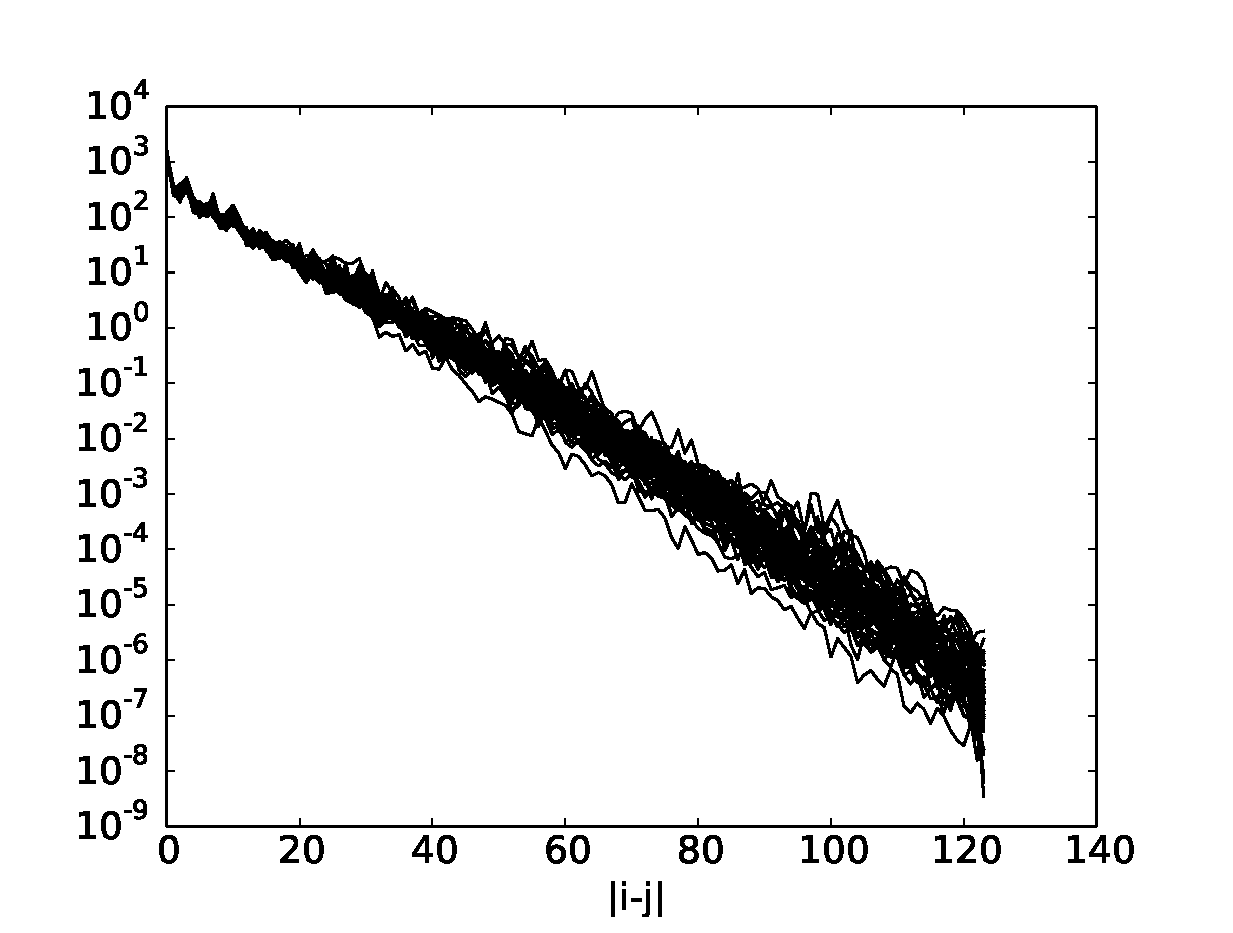
\includegraphics[scale=0.4]{./Figures/HessianDecayLongHorizon.eps}
\caption{Illustration of the off-diagonal decay. Each line corresponds to a different $\lambda$.}
\label{f:HessianDecayLongHorizon}
\end{figure}

\subsection{A short horizon example}

The parameter that seems to have the strongest impact on the decaying is the horizon length. To illustrate this, we generate another random problem with $N=10$, and all other dimensions being the same as before.

The absolute values of the elements in the dual Hessian at the solution $\lambda^*(\tau)$, for $\tau = 1$, are visualized in Figure \ref{f:SpyShortHorizon}. Indeed, there is an evident decay towards the off-diagonal corners, but the relative decay is weaker compared to Figure \ref{f:SpyLongHorizon}. As a consequence, the relative bandwidth of the clipped dual Hessian cannot be made as small before the convergence is seriously hindered.

\begin{figure}[h]
\centering
\includegraphics[scale=0.5]{./Figures/HessianSpyShortHorizon.eps}
\caption{Illustration of the dual Hessian evaluated at $\lambda^*(\tau)$, for $\tau=1$.}
\label{f:SpyShortHorizon}
\end{figure}

As a comparison to Figure \ref{f:ConvergenceLongHorizon}, the convergence for an $m$-banded clipped dual Hessian is visualized, for different values of $m$, in Figure \ref{f:ConvergenceShortHorizon}. Observe that for a certain bandwidth $m$, the convergence is similar for the long and short horizon examples. The difference is, however, that the band is relatively wider in the short horizon case, and accordingly the gain in complexity for using a banded factorization method is smaller. Details of the structural zeros in the clipped dual Hessian for different values of $m$ are summarized in Table \ref{t:StructureShortHorizon}.

\begin{table}[h]
\centering
\caption{Overview of structural zeros in the clipped dual Hessian, for the short horizon example}
\begin{tabular}{c|cccc} \label{t:StructureShortHorizon}
 & Full Hessian & $m=41$ & $m=21$ & $m=11$ \\
 \hline \hline
 Structural zero elements & $0$ & $552$ & $1122$ & $1482$ \\
 Structural nonzero elements & $1936$ & $1384$ & $814$ & $454$ \\
 \hline 
 Ratio of structural zeros & $0\%$ & $28.5\%$ & $58.0\%$ & $76.5\%$ \\ 
\end{tabular}
\end{table}

\begin{figure}[h]
\centering
\includegraphics[scale=0.4]{./Figures/ConvergenceShortHorizon.eps}
\caption{Convergence of Newton and quasi-Newton methods for $\tau=1$.}
\label{f:ConvergenceShortHorizon}
\end{figure}

%\begin{figure}[h]
%\centering
%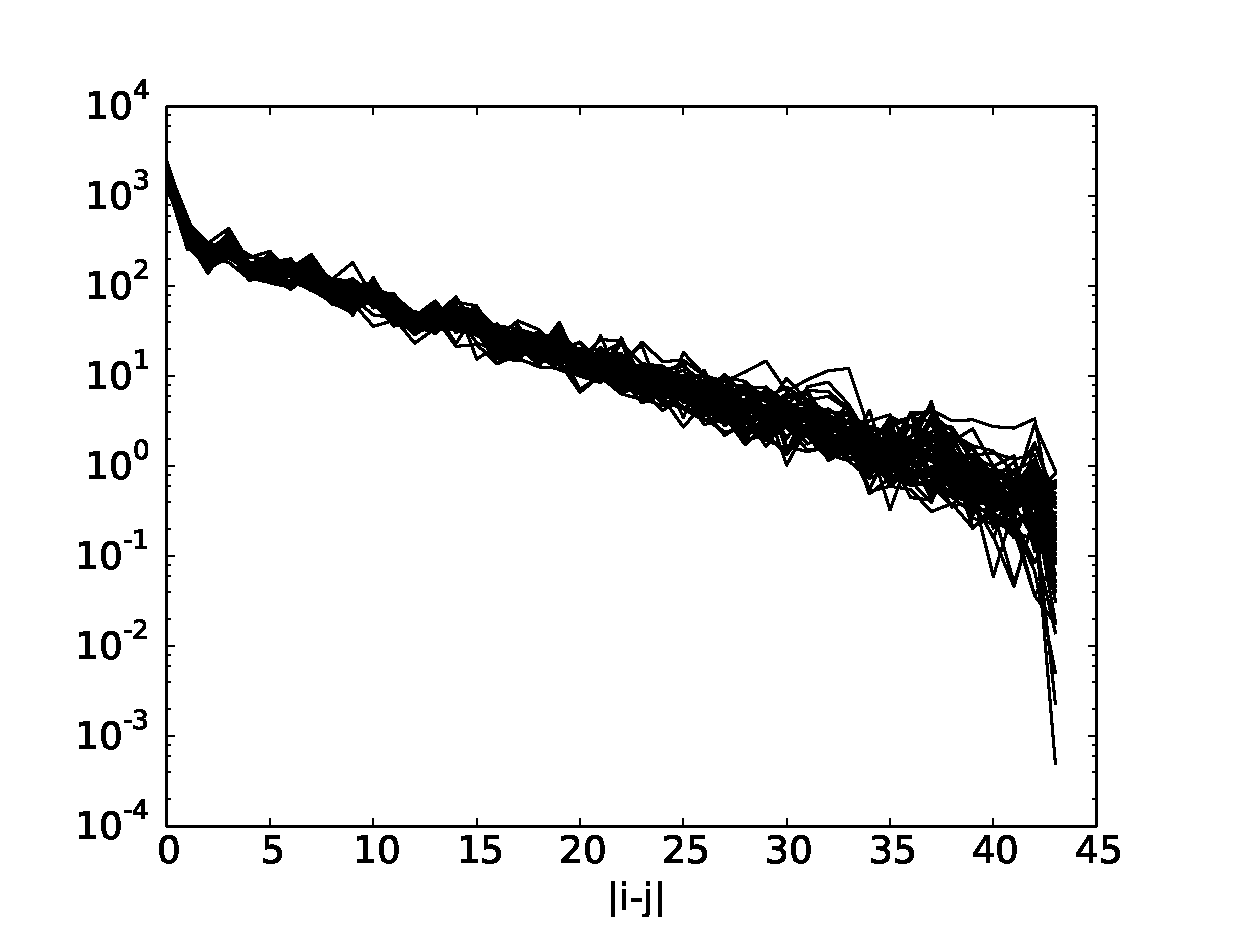
\includegraphics[scale=0.4]{./Figures/HessianDecayShortHorizon.eps}
%\caption{Illustration of the off-diagonal decay. Each line corresponds to a different $\lambda$.}
%\label{f:HessianDecayShortHorizon}
%\end{figure}

%\subsection{An example}
%To investigate the consistency of the off-diagonal decay for a given problem, we look at a randomly generated problem, of the form (\ref{e:problem}), with $M=4$ subproblems each with a horizon $N=30$, $6$ states, $4$ controls, and $4(N+1) = 124$ inequality constraints. At each time instance the subproblems are coupled via $4$ coupling constraints. Moreover, the elements are generated with an even distribution in the interval $[-1000, 1000]$.
%
%The absolute values of the elements in the dual Hessian evaluated at the solution $\lambda^*(\tau)$ for $\tau=1$, are visualized in Figure \ref{f:HessianSpyN30Tau1}. It can be seen that elements with a large magnitude are present along the diagonal, while elements towards the off-diagonal corners are small in absolute value.
%
%\begin{figure}[h]
%\centering
%\begin{subfigure}{.5\linewidth}
%  \centering
%  \includegraphics[width=1\linewidth]{./Figures/HessianSpyN30Tau1.eps}
%  \caption{a) $\tau = 1$}
%  \label{f:HessianSpyN30Tau1}
%\end{subfigure}%
%\begin{subfigure}{.5\linewidth}
%  \centering
%  \includegraphics[width=1\linewidth]{./Figures/HessianSpyN30Tau10minus6.eps}
%  \caption{b) $\tau = 10^{-6}$}
%  \label{f:HessianSpyN30Tau10minus6}
%\end{subfigure}
%\caption{Illustration of the dual Hessian evaluated at $\lambda^*(\tau)$.}
%\label{fig:test}
%\end{figure}
%
%Let us investigate the consistency of the decay with respect to $\lambda$. The maximal absolute value of the elements in $\nabla^2 d(\lambda, \tau)$ for given distances from its diagonal, are visualized in Figure \ref{f:HessianDecayN30Tau1} for 50 randomly selected values of $\lambda$. More specifically, the measure used in Figure \ref{f:HessianDecayN30Tau1} is:
%\begin{equation}
%\begin{aligned}
%\max_{i,j} & \quad | [\nabla^2 d(\lambda,\tau)]_{i,j} | \\
%\text{s.t.} & \quad |i - j| = \text{constant}
%\end{aligned}
%\end{equation}
%Observe that for this example, at all evaluated points $\lambda$, the dual Hessian has a clear decaying trend towards its off-diagonal corners.
%
%\begin{figure}[h]
%\centering
%\begin{subfigure}{.5\linewidth}
%  \centering
%  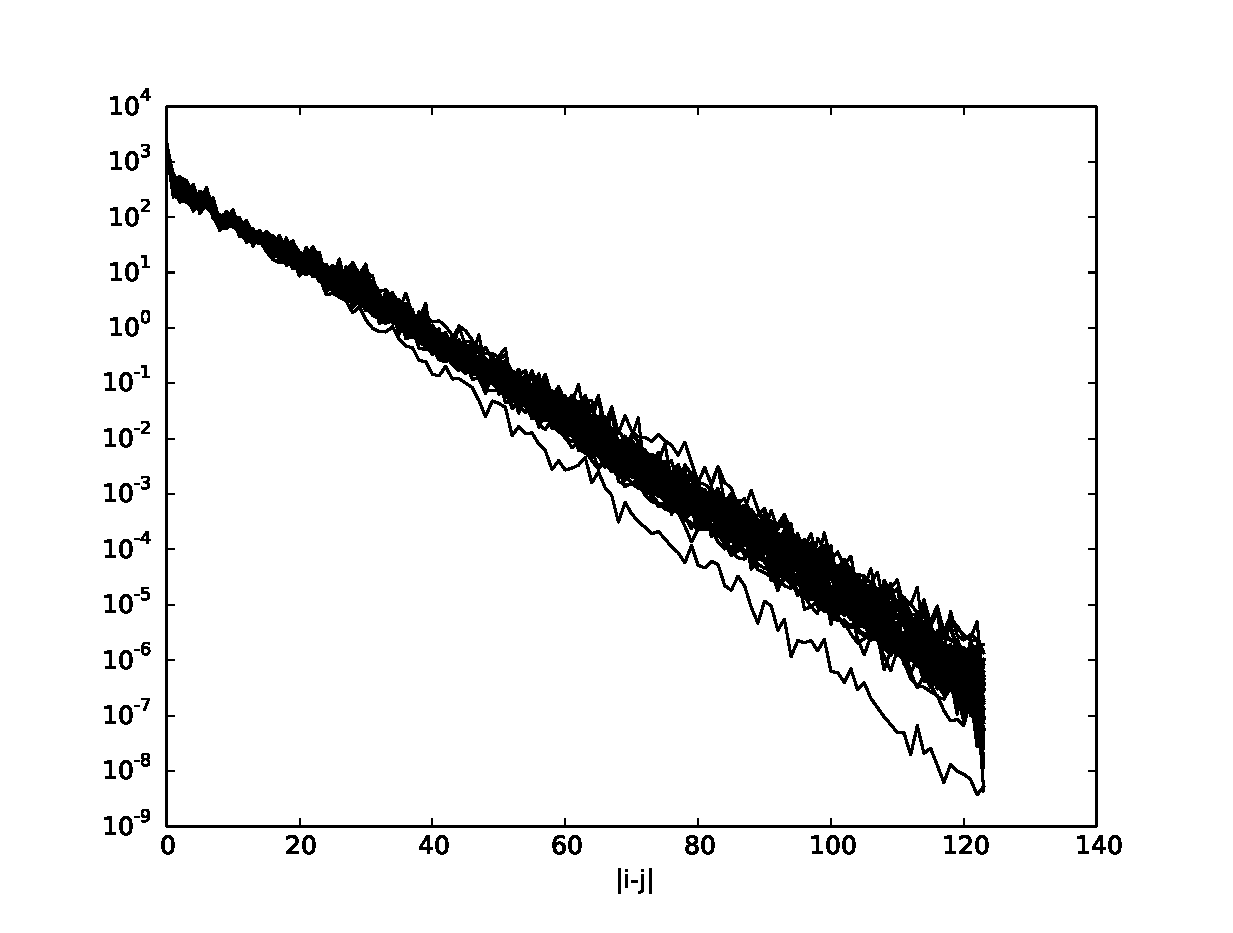
\includegraphics[width=1\linewidth]{./Figures/HessianDecayN30Tau1.eps}
%  \caption{a) $\tau = 1$}
%  \label{f:HessianDecayN30Tau1}
%\end{subfigure}%
%\begin{subfigure}{.5\linewidth}
%  \centering
%  \includegraphics[width=1\linewidth]{./Figures/HessianDecayN30Tau10minus6.eps}
%  \caption{b) $\tau = 10^{-6}$}
%  \label{f:HessianDecayN30Tau10minus6}
%\end{subfigure}
%\caption{Illustration of the off-diagonal decay. Each line corresponds to different $\lambda$.}
%\label{fig:test}
%\end{figure}
%
%As discussed previously, the conditioning of $\Lambda_k$ affects the decaying property and small values of $\tau$ would therefore possibly lead to a slower decay. Corresponding figures to Figure \ref{f:HessianSpyN30Tau1} and Figure \ref{f:HessianDecayN30Tau1}, for $\tau = 10^{-6}$, are shown in Figure \ref{f:HessianSpyN30Tau10minus6} and Figure \ref{f:HessianDecayN30Tau10minus6} respectively. Observe that, for this example, there is no significant difference in the decay between the different values of $\tau$. This observation pertain to all experiments we have seen so far.
%
%The parameter that seems to have the strongest impact on the decaying is the horizon length. To illustrate this, we generate another random problem with $N=10$, and all other dimensions being the same as before. The dual Hessian at the solution $\lambda^*(\tau)$, for $\tau=1$ is visualized in Figure \ref{f:HessianSpyN10Tau1}. Observe that the dual Hessian also in this case has a clear decay towards the off-diagonal corners. The band with elements of a significant magnitude is however wider compared to the size of the matrix. Moreover, the decaying property is visualized for $50$ different values of $\lambda$ in Figure \ref{f:HessianDecayN10Tau1}. Note that in this figure it is easier to see that there is a smaller difference between the diagonal and the off-diagonal elements.
%
%\begin{figure}[h]
%  \centering
%  \includegraphics[scale=0.4]{./Figures/HessianSpyN10Tau1.eps}
%  \caption{Illustration of the dual Hessian evaluated at $\lambda^*(\tau)$.}
%  \label{f:HessianSpyN10Tau1}
%\end{figure}
%
%\begin{figure}[h]
%  \centering
%  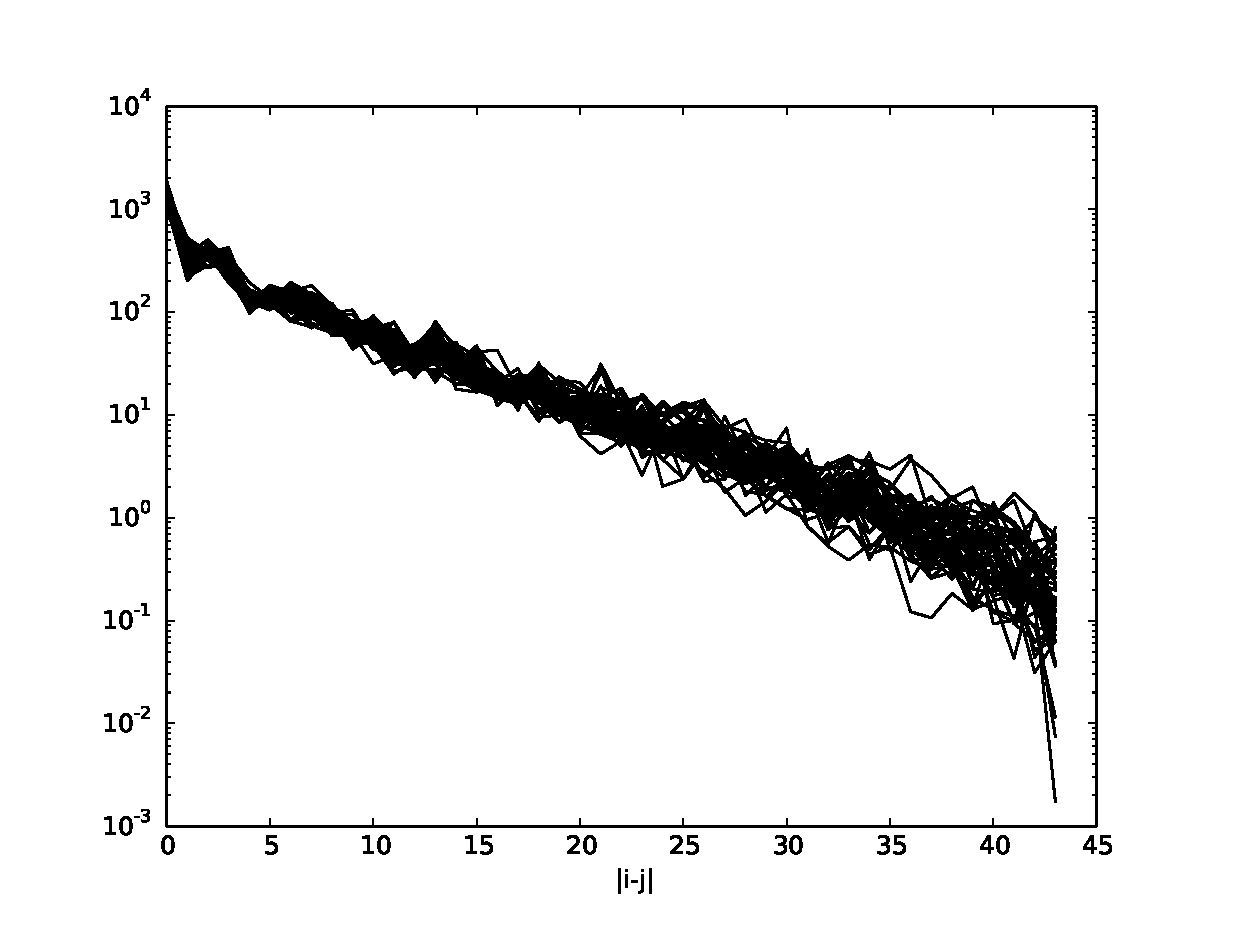
\includegraphics[scale=0.4]{./Figures/HessianDecayN10Tau1.eps}
%  \caption{Illustration of the off-diagonal decay. Each line corresponds to different $\lambda$.}
%  \label{f:HessianDecayN10Tau1}
%\end{figure}


\section{Conclusions} \label{S:Conclusions}

This paper is devoted to showing that the Hessian of the dual function originating from many distributed MPC problems possess a quasi-banded structure. Due to the quasi-structure, a banded approximation of the Hessian can be formed, for which structure exploiting factorization methods can be used. We show that the structure can be used to form a quasi-Newton method, which can solve problems of the considered class to a lower overall complexity compared to a Newton method.

The quasi-structure is analyzed in the context of the interior-point methods presented in \cite{Necoara2009a}, \cite{Quoc2013} and \cite{Klintberg2014}. However, we also show that the structure is present in active-set methods.

By numerical experiments, we showed that the quasi-structure is strong especially for MPC problems with a very long horizon. In those cases, it is often possibly to find a good approximation of the Newton direction by only considering a small fraction of the elements in the dual Hessian. This should be very appealing for systems with fast and slow dynamics, e.g. power grids with storage capabilities. 


%\begin{acknowledgements}
%If you'd like to thank anyone, place your comments here
%and remove the percent signs.
%\end{acknowledgements}

% BibTeX users please use one of
%\bibliographystyle{spbasic}      % basic style, author-year citations
\bibliographystyle{spmpsci}      % mathematics and physical sciences
%\bibliographystyle{spphys}       % APS-like style for physics
%\bibliography{}   % name your BibTeX data base

% Non-BibTeX users please use
\bibliography{optec}

\end{document}
% end of file template.tex

